\subsection{Исходное изображение}

Для последнего задания выберем следующее изображение:

\begin{figure}[ht!]
    \centering
    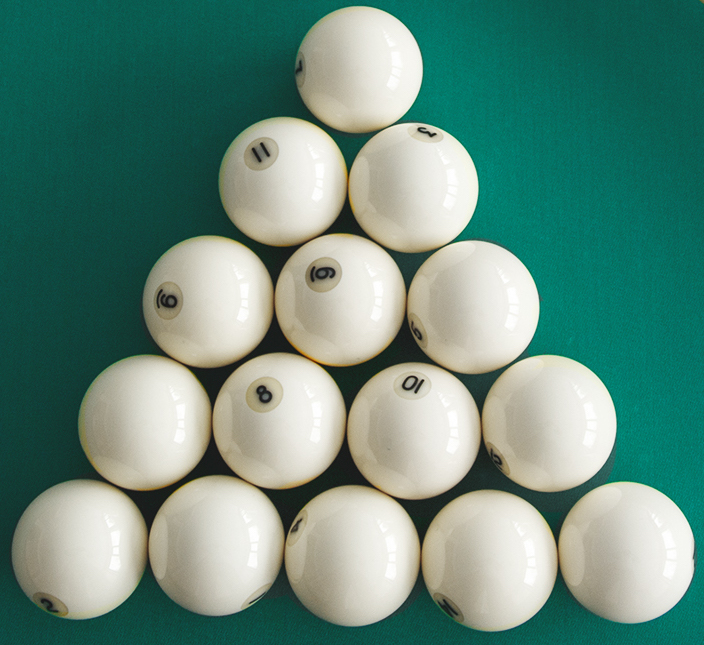
\includegraphics[width=0.8\textwidth]{images/source_images/snooker.jpg}
    \caption{Шары для игры в бильярд}
    \label{img:billiard_balls}
\end{figure} 

\subsection{Программа на языке Python}
\begin{lstlisting}[caption={Исходный код программы для сегментации изображения}, label={lst:separation}]
    def bwareaopen(image, dim, conn=8):
        assert image.ndim == 2, None
        # Find all connected components
        num, labels, stats, centers = cv.connectedComponentsWithStats(image, connectivity=conn)
        # Check size of all connected components
        for i in range(num):
            if stats[i, cv.CC_STAT_AREA] < dim:
                image[labels == i] = 0
        return image


    # loading an image
    src_img = cv.imread('source_images/snooker.jpg')
    # converting it to binary
    gray_img = cv.cvtColor(src_img, cv.COLOR_BGR2GRAY)
    ret, i_bw = cv.threshold(gray_img, 0, 255, cv.THRESH_BINARY + cv.THRESH_OTSU)
    # deleting tiny connected components
    i_bw = bwareaopen(i_bw, 20, 8)
    disk = cv.getStructuringElement(cv.MORPH_ELLIPSE, (5, 5))
    i_bw = cv.morphologyEx(i_bw, cv.MORPH_CLOSE, disk)
    # display_image('Binary_closed', i_bw, 1)

    # finding foreground
    i_fg = cv.distanceTransform(i_bw, cv.DIST_L2, 5)
    ret1, i_fg = cv.threshold(i_fg, 0.6 * i_fg.max(), 255, 0)
    i_fg = i_fg.astype(np.uint8)
    ret2, markers = cv.connectedComponents(i_fg)
    # display_image('Fg', i_fg, 1)


    # Find background location
    i_bg = np.zeros_like(i_bw)
    markers_bg = markers.copy()
    markers_bg = cv.watershed(src_img, markers_bg)
    i_bg[markers_bg == -1] = 255
    # display_image('Bg', i_bg, 1)

    # Define undefined area
    i_unk = cv.subtract(i_bg, i_fg)
    # Define all markers
    markers = markers + 1
    markers[i_unk == 255] = 0
    # Do watershed
    # Prepare for visualization
    markers = cv.watershed(src_img, markers)
    # display_image('UND', i_unk, 1)
    markers_jet = cv.applyColorMap((markers.astype(np.float32)*255/(ret2 + 1)).astype(np.uint8), cv.COLORMAP_JET)
    display_image('Jet_fg_markers', markers_jet, 1)
    src_img[markers == -1] = (0, 0, 255)
    # display_image('result', src_img, 1)
\end{lstlisting}

\subsection{Результат}

Для начала необходимо получить бинарное изображение, предварительно удалив лишние детали.

\begin{figure}[ht!]
    \centering
    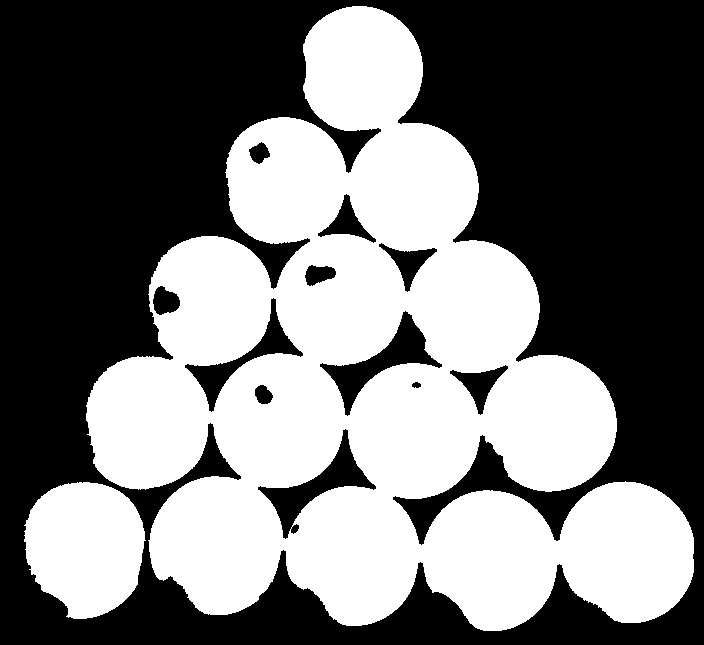
\includegraphics[width=0.7\textwidth]{images/transformed_images/3/Binary_closed.jpg}
    \caption{Бинарное изображение}
    \label{img:bin_balls}
\end{figure} 

Далее воспользуемся преобразованием евклидова расстояния и после дополнительной фильтрации получим маркеры переднего плана:

\begin{figure}[ht!]
    \centering
    \begin{subfigure}{0.4\textwidth}
        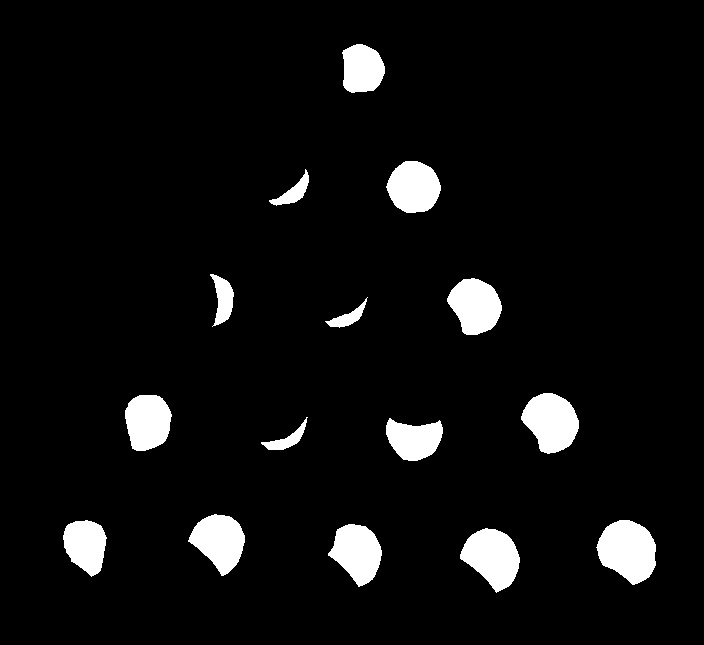
\includegraphics[width=\textwidth]{images/transformed_images/3/Fg.jpg}
        \caption{}
        \label{img:bin_fg}
    \end{subfigure}
    \begin{subfigure}{0.4\textwidth}
        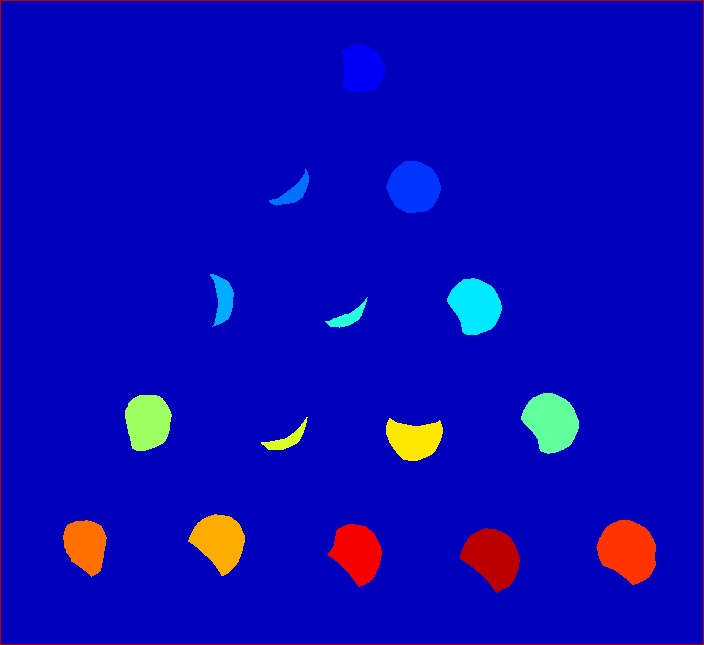
\includegraphics[width=\textwidth]{images/transformed_images/3/Jet_fg_markers.jpg}
        \caption{}
        \label{img:jet_fg}
    \end{subfigure}
    \caption{Определение маркеров переднего плана: (a) область маркеров переднего плана, (b) маркеры переднего плана}
    \label{img:FG}
\end{figure} 

Далее получим маркеры фона и неопределенной области:

\begin{figure}[ht!]
    \centering
    \begin{subfigure}{0.4\textwidth}
        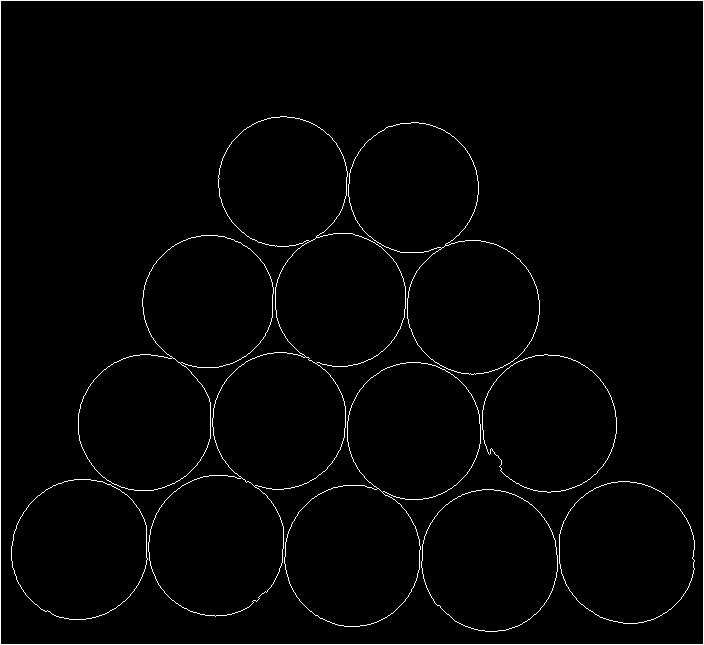
\includegraphics[width=\textwidth]{images/transformed_images/3/Bg.jpg}
        \caption{}
        \label{img:bin_bg}
    \end{subfigure}
    \begin{subfigure}{0.4\textwidth}
        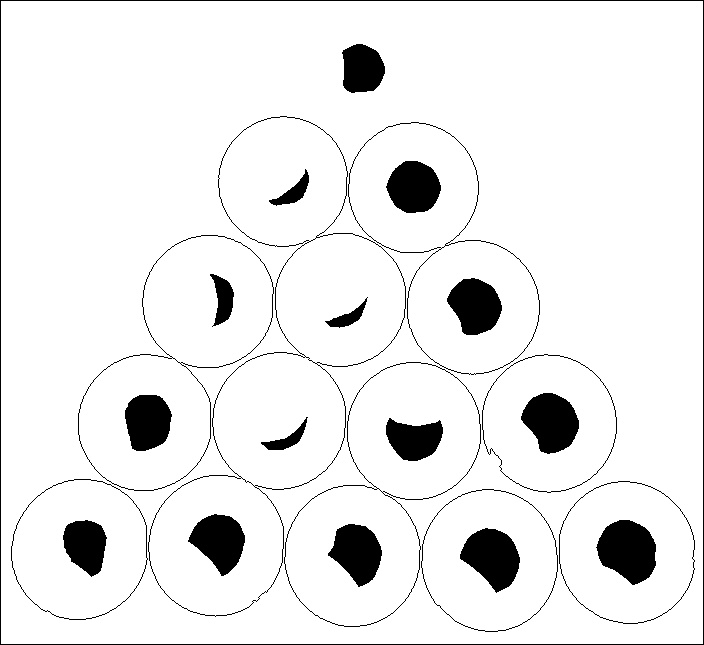
\includegraphics[width=\textwidth]{images/transformed_images/3/UND.jpg}
        \caption{}
        \label{img:bin_und}
    \end{subfigure}
    \caption{Определение маркеров: (a) фона, (b) неопределенной области}
    \label{img:BG}
\end{figure} 

Наконец, получим результаты сегментации:

\begin{figure}[ht!]
    \centering
    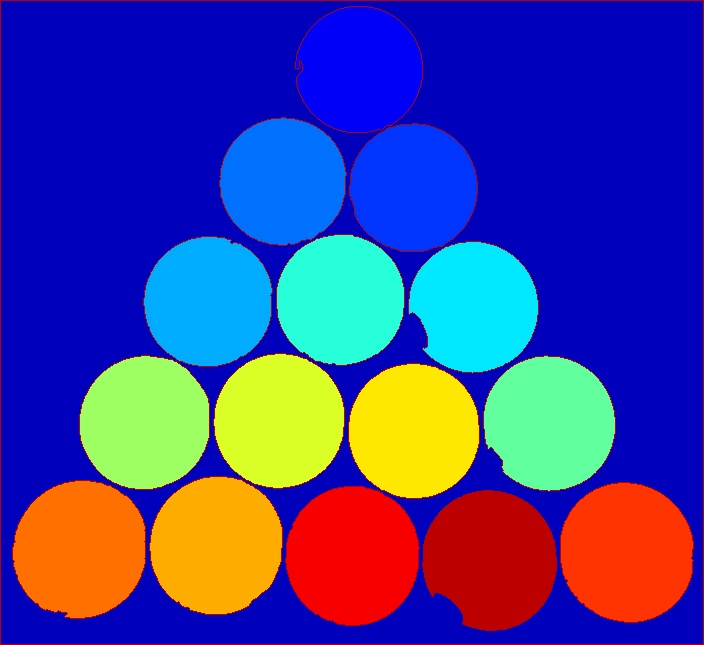
\includegraphics[width=0.7\textwidth]{images/transformed_images/3/Jet.jpg}
    \caption{Результат сегментации}
    \label{img:seg}
\end{figure} 
\clearpage
\begin{figure}[ht!]
    \centering
    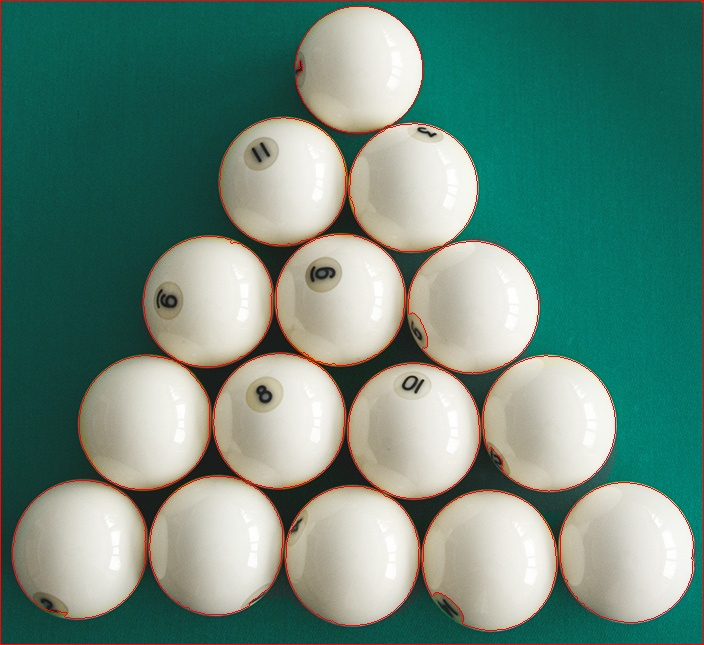
\includegraphics[width=0.7\textwidth]{images/transformed_images/3/result.jpg}
    \caption{Результат сегментации, наложенный на исходное изображение}
    \label{img:seg_orig}
\end{figure} 